\chapter{Dynamic OpenCL}
\label{main}
In this chapter the conceived and implemented framework, called Dynamic OpenCL, is explained. Section \ref{distribution} discusses the options for the underlying distribution technologies, including benchmarks to prove the feasibility of the final choices. In section \ref{abstraction} the utilized high-level abstraction of OpenCL code is introduced, portraying contributions to existing software solutions. Based on these explanations section \ref{job_design} contains insight into the defined job structure for parallelization within Dynamic OpenCL. The remaining sections about \textit{\nameref{main_hybrid_cloud}}, \textit{\nameref{scalable_performance}} and \textit{\nameref{optimized_scheduling}} cover solutions for flexible resource adjustments and performance improvements in shared environments. The resulting framework code as well as modified dependencies can be found by accessing the repository links given in section \ref{appendix:links} of the appendix.

\section{Distribution Approach}
\label{distribution}
As portrayed in section \ref{distribution_basics} and \ref{related} many viable options exist to distribute tasks among devices within a single machine as well as across a cluster. This section will explain the reasons for selecting the fitting approaches based on the goals declared in section \ref{goals}. The options are considered based on different levels of parallelization, depicted in figure \ref{img:parallelization_levels}. Following this structure the final solution should be able to parallelize across connected clusters, machines within a cluster, multiple devices within a machine and ultimately across all available device cores.

\begin{figure}[H]
	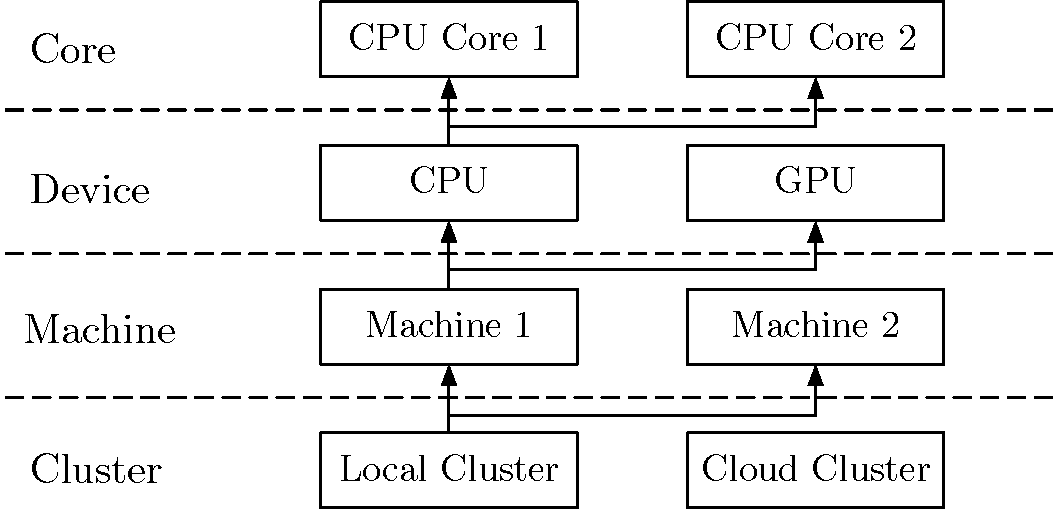
\includegraphics[width=0.55\textwidth]{drawings/parallelization_struct.pdf}
	\centering
	\caption{Levels of Parallelization}
	\label{img:parallelization_levels}
\end{figure}

As a first step the options for parallelization on multiple device cores are considered. Low level solutions like OpenMP or OpenACC are matured and known for simple mechanisms to parallelize portions of a program. While programmers are given freedom to utilize available directives according to their demands, this also increases the risk for programming errors especially in more complex scenarios. \citeauthor{openmp_mistakes} have shown that novice OpenMP programmers tend to make common mistakes regarding correctness and performance in small and medium-sized programs\cite{openmp_mistakes}. Programmers are thus not only mandated to understand the OpenMP specification but also to choose the right set of directives for the respective problem. When targeting accelerators the same learning process has to be undertaken for the OpenACC specification. As all communication and synchronization across multiple cores and devices has to be handled by the programmer, a significant layer of complexity through the utilization of code directives is introduced. 

Computing frameworks like OpenCL and CUDA offer this level of parallelization through a fixed programming model, which dictates a standardized form in which algorithms have to be designed. For example, OpenCL proposes the creation of Kernels that follow an execution model based on work-groups and work-items. While CUDA offers similar capabilities as OpenCL, it only supports NVIDIA GPUs and lacks CPU support. This contradicts with the proposed goal of a heterogeneous environment in which devices of different types and vendors cooperate. Therefore OpenCL is chosen for multi-core parallelization.

OpenCL additionally allows to distribute programs to multiple devices without changes to the code. It even enables parallel computation by multiple devices as long as all participating devices belong to the same OpenCL platform, which in practice describes the hardware vendor. Thus multiple NVIDIA GPUs can share data and corresponding executions. For a heterogeneous cluster this approach is insufficient as various CPUs and GPUs are required to cooperate. In order to enable sharing workloads across varying devices a dedicated solution is presented throughout this chapter.

For distributing partial tasks across a cluster many solutions are available. Though most require significant cluster management or programming efforts. As OpenCL is selected as the underlying computational framework per machine, the cluster distribution technology has to fit its capabilities.
Similar to OpenMP, MPI has matured over decades as a standard solution for low level communications between multiple machines. As such it has also been used frequently in conjunction with OpenCL and has inspired frameworks based on this combination. As the MPI standard spans over 800 pages, covering more than 300 functions\cite{mpi_spec}, significant knowledge of the API is required in order to build correct and performant processes. As such MPI adds noticeable program complexity to existing OpenCL programs.

On the opposite MapReduce based frameworks like Hadoop MapReduce offer a strict programming model with a fixed form to follow for each implemented algorithm. Multiple research projects cover the usage of OpenCL in conjunction with MapReduce, proving its feasibility\cite{hadoopcl}\cite{hadoop+}. Hadoop MapReduce requires an underlying distributed file system like HDFS, which increases management efforts as not only MapReduce nodes but also file system nodes have to be maintained within the cluster. Additionally, Hadoop MapReduce spawns a JVM for each worker process, thus introducing startup overheads and increasing memory usage.

While many of the previously described cluster distribution approaches are used in professional projects, other solutions exist that can circumvent the prevalent issues. OpenCL API forwarding libraries, as shown in section \ref{cluster_distribution}, can offload computational workloads to remote machines within a cluster without impacting programmers or requiring significant cluster management. Instead they wrap the execution and handle network communication and data transfers transparently while only requiring a running demon on a remote machine. Additionally API forwarding allows to send computations to distant clusters as long as a connection to the sending machine exists.

The considered forwarding libraries include SnuCL, VirtualCL and dOpenCL. While all mentioned solutions introduce certain specialties, the key feature to be considered is the API forwarding, which has to work stable in order to ensure a well functioning distribution of tasks. Therefore as a first step the three frameworks are installed on several machines of Type A and B, which are presented in \ref{cluster_composition}.

Every framework is installed following its respective included documentation. In the case of SnuCL the installation can not be completed on the respective systems using the two newest versions 1.3.2 and 1.3.3. While VirtualCL 1.24 can be installed without issues, executing various OpenCL programs leads to inconsistent Segmentation Faults. The last candidate, dOpenCL 0.4.0r1819, can be installed successfully and manages to run all tested programs without issues, even those that previously failed for VirtualCL. Therefore dOpenCL is chosen for more detailed benchmarks to investigate performance caveats.

Due to its architecture, dOpenCL has to communicate back and forth with remote devices over the network in order to send inputs and retrieve results. Thus, computations can be highly impacted by network transfers when the algorithm performs relatively quickly in comparison to the data sizes. To evaluate these impacts a matrix multiplication is executed on a cluster consisting of machines of Type A and B. As the general equation of a matrix multiplication is $AB = C$, the two input matrices have to be transferred to the executing device and the resulting matrix has to be retrieved after completing the computation. This means that three data transfers have to be made, which in the case of a $8000x8000$ float matrix is $8000^2 * 4\ Bytes = 256\ Megabytes$. For a perfect 1 Gbit/s connection without TCP overhead transferring the three matrices might take $3*256\ Megabyte / 125\frac{Megabyte}{s} = 6.1s$. In order to distinguish the computational time from the data transfer times, data transfers are measured utilizing the OpenCL profiling options. The algorithm is run for varying problem sizes on a cluster consisting of multiple machines of Type A and B. It is first run locally without dOpenCL on a machine of each type and then remotely from a second machine.

\begin{figure}[!htb]

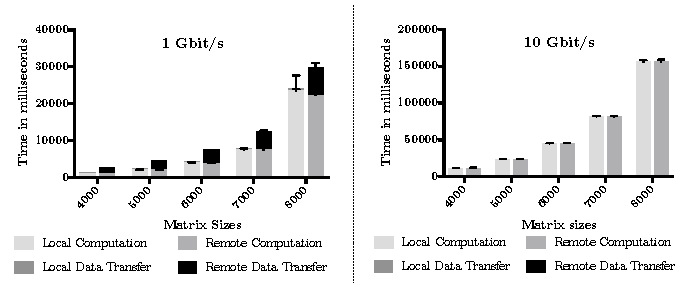
\includegraphics[width=1.0\textwidth]{images/data_transfer.pdf}
\centering
\caption{dOpenCL Benchmark Remote vs. Local}
\label{img:data_transfer}
\end{figure}

It is visible from the obtained results in figure \ref{img:data_transfer} that the local executions have minimal transfer times for the matrices as their only limiting factor is the bus interface between CPU and RAM. On the opposite, data transfers can have significant impact on performance for remote executions as the Ethernet transfers have to be added on top the mandatory bus transfers. This is especially true for fast machines that only have an inadequate interconnection speed like Type A. While for matrix sizes of 8000x8000 the local execution only requires less than 2\% of the time for data transfers, its remote counterpart uses 25\% of the total for these operations. In the case of Type B, the remote transfers profit from the 10 Gbit/s interconnect. As Type B is considerably slower than Type A during the computation phase, the fraction of data transfer time lies around 1\% of the total time, which is negligible.

Based on the results, one can conclude that the remote computation itself is nearly as fast as the local execution and that the introduced overhead by dOpenCL is marginal. Real performance degradations occur when data transfers have to be processed, which are directly affected by the network performance. Still, dOpenCL can greatly improve performance when accessing a superior machine via remote as seen in the example of Type A and Type B. For the given workload Type A could provide a 5x speedup to Type B if it outsourced its computations of 8000x8000 matrices.

Concluding the findings and design decisions a framework named Dynamic OpenCL is proposed. An overview over the architecture is shown in figure \ref{img:dynamic_opencl_arch}. In its center works a \textit{Management Node} that runs the Dynamic OpenCL library in conjunction with dOpenCL. The library is among other things responsible for code abstractions and scheduling services, which are explained throughout this chapter. The management node is connected to several \textit{Compute Nodes} through dOpenCL, which have the dOpenCL daemon running. Using the connection the management node distributes tasks to remote devices located in the local cluster or provided by cloud services.

\begin{figure}[H]

	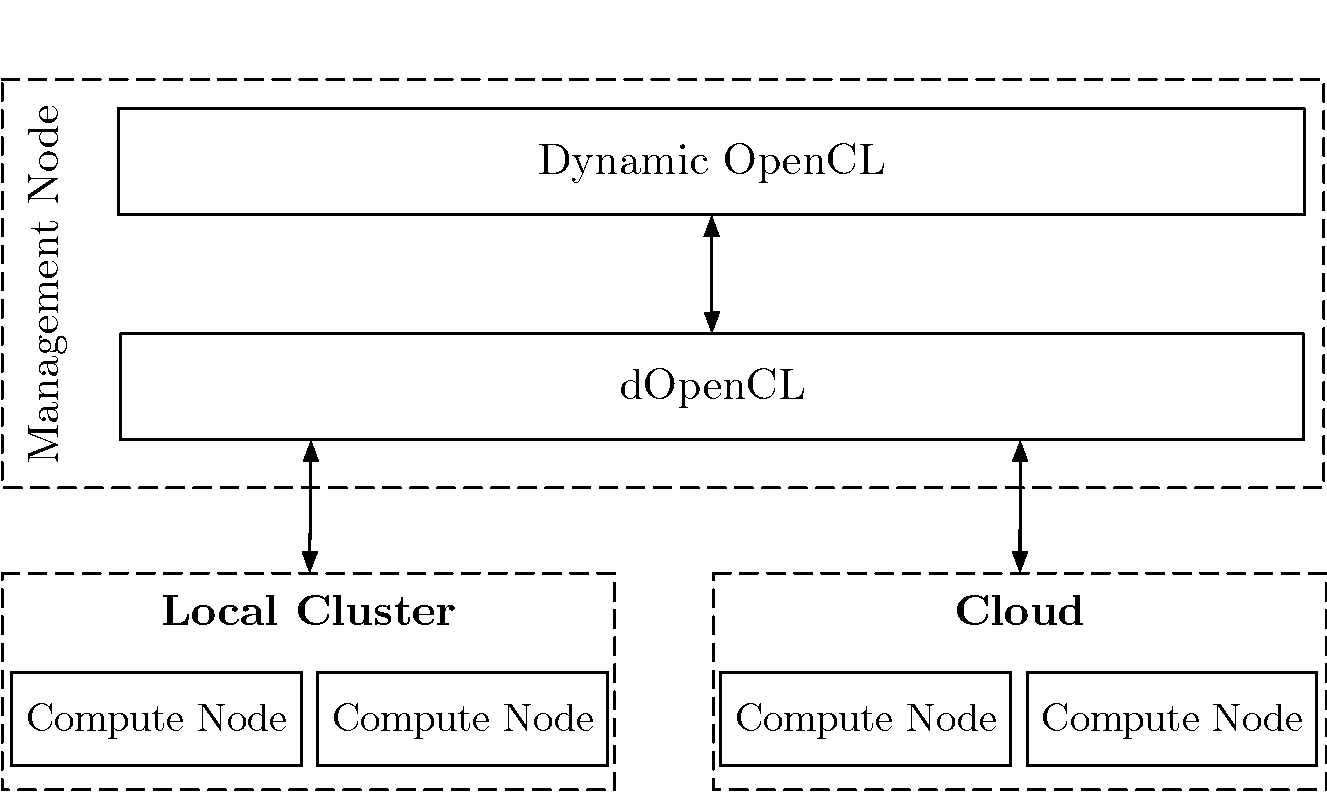
\includegraphics[width=0.7\textwidth]{drawings/dynamic_opencl_arch.pdf}
	\centering
	\caption{Dynamic OpenCL Architecture}
	\label{img:dynamic_opencl_arch}
\end{figure}

\section{High-Level Abstraction}
\label{abstraction}

In section \ref{aparapi} it was shown how little code and knowledge of internals are required for building OpenCL computations with the help of Aparapi. Including the library in the final framework would not only benefit end users due to a simplified programming environment but also greatly assist during the creation of the framework itself. Through Aparapi, Java could be used as the overall project language while abandoning C++ for most parts with the exception of dOpenCL and Aparapi internals. Due to the choice of a more high level language for the less performance critical code, Java promises faster building time and better maintainability. In order to achieve this, Aparapi has to be connected to dOpenCL to harness the distribution capabilities. First, it has to be evaluated, whether Aparapi performs adequately compared to an original OpenCL algorithm. For that cause the matrix multiplication benchmark from section \ref{distribution} is transformed to Aparapi and executed on a machine of Type B from the benchmark cluster. As Aparapi translates the Java code for Kernels it has not encountered before, the translation time would skew the results for the first iteration of a run. Therefore at first the average translation time for differently sized Kernels is measured on a machine of Type B with 100 iterations per Kernel, depicted in \ref{img:aparapi_translation}.

\begin{figure}[H]
	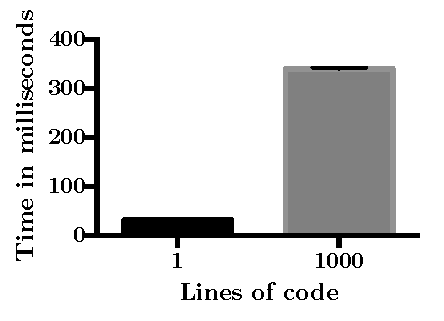
\includegraphics[width=0.35\textwidth]{images/aparapi_translation.pdf}
	\centering
	\caption{Average Kernel translation time}
	\label{img:aparapi_translation}
\end{figure}

It is visible that the translation time of a kernel has a lower bound of ~30ms on machines of Type B. Additionally it can be concluded that the translation time is correlated to the Kernel size but even for many lines of code remains at around 350ms. In the light of long running computations this time becomes diminishable. Another reason for slow execution times of a first Kernel run is the lazy initialization feature of Aparapi's execution engine. This means that Aparapi internals like native libraries are not loaded until the first Kernel is submitted. Because these initial execution costs shall be ignored in the final results, an initial warmup run is executed to initialize the execution engine as well as to cache the translated OpenCL code. The matrix sizes as well as the number of iterations remain identical to the benchmark from section \ref{distribution}.

\begin{figure}[H]
	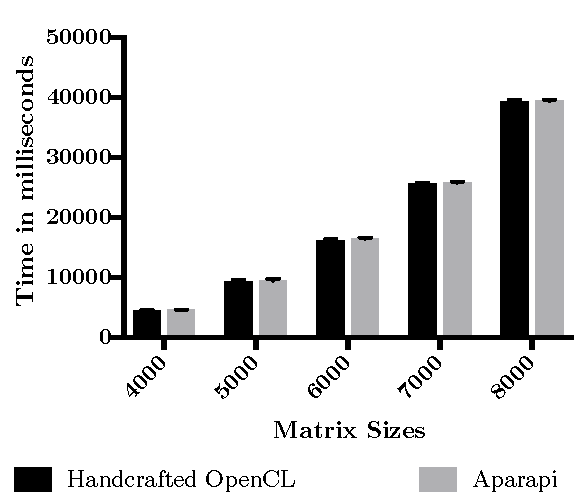
\includegraphics[width=0.7\textwidth]{images/aparapivsopencl.pdf}
	\centering
	\caption{Aparapi vs. Handcrafted OpenCL}
	\label{img:aparapi_vs_opencl}
\end{figure}

As visible in the results in figure \ref{img:aparapi_vs_opencl}, Aparapi can reach the performance level of handcrafted OpenCL code, which for the measured problem sizes takes less than 2\% longer to compute. This minuscule difference could be the result of communication overhead through the JNI interface. Because of the similar performance it is valid to utilize Aparapi in the envisioned framework. As a first step the connection between Aparapi and dOpenCL should be evaluated. For this cause both components are installed on a development system and tested for interoperability. It is discovered that in their standard versions both pieces of software do not work in conjunction because of several bugs or incompatible design decisions. These problems and the corresponding solutions are explained in the following part.

\section*{Contributions to Aparapi and dOpenCL}
\begin{description}[style=nextline]
	\item [No available devices]
	When querying dOpenCL for appropriate devices from Aparapi, none are returned even though multiple devices are available when using standard OpenCL. The problem for this symptom lies within dOpenCL, which insufficiently implements the query method. OpenCL uses a single byte to identify queried devices types. For instance \textit{00000010} queries CPUs and \textit{00000100} asks for GPUs. dOpenCL checks for the position of the positive bit and correctly returns devices of the requested type. In fact the OpenCL specification also allows bitwise OR-operations on multiple types so that when requesting for CPUs and GPUs in one query: \textit{00000010 OR 00000100 = 00000110}. As Aparapi only supports CPUs and GPUs, it specifically utilizes this byte even when the user only requests a CPU. The actual filtering is then done in Aparapi's Java code. Because dOpenCL does not support these combined queries, it can not return any devices to Aparapi. Therefore this method is fixed, which results in Aparapi successfully obtaining information about available devices.

	\item [Specific device choice]
	Aparapi by design is focused on providing a simple API, which lacks certain features that are important for Dynamic OpenCL. For example it is desirable to have multiple instances of the same Kernel run in parallel with different data. Therefore it would be possible to split tasks into smaller subsets of data that could be distributed to various devices. Aparapi allows to define preferences on which specific device a Kernel should be run. This preference is saved on class level instead of instance level, which means that all instances of the same class would be directed to the same device. Therefore no parallelization is possible with the standard Aparapi version. In order to fix this issue, the mechanism for memorizing preferences is modified to respect the definitions for each individual instance of a Kernel.

	\item [Failed compilations when using multiple devices]
	Due to fixing the previously described issues, the development system is able to successfully execute Kernels on a single node cluster. Adding a second machine with different installed devices produces an error during the OpenCL compilation process even when only one device is targeted for execution. In the given environment both nodes by itself are able to compile the Kernel without any incidents. Additionally it is verified that dOpenCL without Aparapi supports the multi node cluster. Therefore it is suspected that Aparapi has a bug that prevents the compilation when more than one machine is present. Through reviewing Aparapi internals the cause for the issue is found: Aparapi creates an OpenCL context not per device but per type. OpenCL contexts serve for sharing memory and control structures between multiple devices but can only be defined for devices of the same platform. Thus, when having multiple CPUs of different vendors in a cluster, Aparapi tries to create a context for all CPUs, which creates the error. In order to prevent this violation, in the fixed version contexts are created only for a single device.

	\item [Multiple platforms per machine]
	Systems that run OpenCL can support multiple platforms in parallel. For example, a machine that has an Intel CPU as well as a NVIDIA GPU installed offers two platforms. For a node with such a setup dOpenCL only recognizes the first platform, namely Intel, and ignores the NVIDIA platform. Reviewing the code reveals that this is indeed a fixed behavior in the code that by default only passes on the first found platform of a system. In order to support systems with multiple platforms at hand this code is reworked to recognize all available platforms.

\end{description}


\section{Job Design}
\label{job_design}
With the implemented fixes described in section \ref{abstraction} Aparapi is able to successfully communicate with dOpenCL and deploy tasks to multiple remote devices. This ability enables jobs to be split up into subtasks, which can be computed in parallel. Therefore the envisioned framework has to provide a mechanism for submitting split tasks by the programmer. With such a mechanism the challenge arises how to distribute data among splits. While some problems may have no or little dependency across data, others may require complex interconnections between individual data points. Thus it is inevitable to ensure that each split has all the necessary data for its correct computation. On the opposite, naively including the full data set in each split may lead to serious performance penalties due to longer data transfer times. This becomes especially important with the introduction of remote execution libraries like dOpenCL, where the most likely bottleneck is the network connection. Based on previous research the following methods are identified:

\begin{description}[style=nextline]
	\item [Manual Splits]
	Hadoop MapReduce enforces saving input data for the executable tasks in split files on the Hadoop Distributed File System. Each split file is executed independently and programmers have to define how to interpret a split during the map phase. Ultimately, the individually programmed reduce algorithm merges the splits together to form a final result.

	\item [Naive Buffer Replication]
	A simple and safe way to ensure that every split has the required data available is to transfer all data to the employed devices as done by \citeauthor{delalama_2012}\cite{delalama_2012}. Their method of buffer replication is trivial when transferring to the devices. On the opposite merging the individual output buffers back into the final result requires an algorithm to determine the parts that should be included by each split.

	\item [Intelligent Buffer Replication]
	\citeauthor{Kim_2011}\cite{Kim_2011} have developed a mechanism to automatically determine how to split input buffers among subtasks in OpenCL so that only minimal data has to be transferred. Their method is based on sampling memory access patterns before sending the data so that lower and upper memory bounds can be determined.

	\item [Meta Functions]
	\citeauthor{stepocl}\cite{stepocl} as well as \citeauthor{distcl}\cite{distcl} employ meta functions that are utilized to determine split data independent from the problem size. These meta functions have to be supplied by the programmer and define the memory access patterns by the algorithm.

\end{description}

While all of the above mentioned methods are meaningful candidates, they each have negative impact either on performance or programming complexity: \textit{Naive Buffer Replication} increases total data transfer sizes, which enhances the chances of network congestion the higher the number of splits becomes. \textit{Intelligent Buffer Replication} requires an extra step for sampling memory accesses, which includes the translation of OpenCL to C code. Although \textit{Meta Functions} try to abstract efforts away from programmers they are still required to define the access patterns manually. \textit{Manual Splits} put the entire responsibility into the hands of the programmer who has to make sure that the data is split and merged back together. While it is the least automated method, it also grants full control over performance and is not dependent on split and merge algorithms that may fail for complex problems. Thus, the framework supports \textit{Manual Splits}. In order to show that such an approach is eligible in combination with Aparapi Source Code \ref{lst:split_addition} illustrates the process of splitting the addition of two vectors into partial tasks.


\begin{lstlisting}[caption=Partial Aparapi Vector Addition Kernel,captionpos=b,label=lst:split_addition]
public class AdditionKernel extends Kernel{
  int[] a, b, result;

  public AdditionKernel(int[] a, int[] b) {
    this.a = a;
    this.b = b;
    this.result = new int[a.length];
  }

  @Override
    public void run() {
    int i = getGlobalId();
    result[i] = a[i] + b[i];
  }
}

public class Addition {
  public static void main(String[] args) {
    final int partialCount = 2;
	int[] a = new int[]{0, 1, 2, 3, 4, 5, 6, 7, 8, 9};
	int[] b = new int[]{0, 1, 2, 3, 4, 5, 6, 7, 8, 9};
	int[] result = new int[a.length];
	
	int partialWidth = a.length / partialCount;
	for(int i = 0; i < partialCount; i++){
      int[] aPartial = Arrays.copyOfRange(a, i * partialWidth, (i + 1) * partialWidth);
      int[] bPartial = Arrays.copyOfRange(b, i * partialWidth, (i + 1) * partialWidth);
	
	  AdditionKernel additionKernel = new AdditionKernel(aPartial, bPartial);
      additionKernel.execute(partialWidth);
      System.arraycopy(additionKernel.result, 0, result, i * partialWidth, partialWidth);
	}
	
	System.out.println(Arrays.toString(result));
  }
}

\end{lstlisting}

In the example a reusable Aparapi Kernel \textit{AdditionKernel} is defined that computes the sums of the two vectors independent of the general problem size. In the class \textit{Addition} the generated input data is split into smaller parts based on the \textit{partialCount}. Then for each partial the \textit{AdditionKernel} is instantiated and executed. After the execution the individual result is copied into the overall \textit{result} array. In order to grant higher parallelization the \textit{tileCount} could be dynamically changed into a divisor of the array length. This illustrates that writing a split and merge algorithm can be intuitive and not require much code.

Based on the above explanations the following execution model for Dynamic OpenCL is defined, which is depicted in \ref{img:dynamic_opencl_job}. Users define \textit{Jobs}, which are comprised of at least one \textit{Partial}, which is an extended Aparapi Kernel. Partials contain the data that is split manually. After a job is constructed it can be submitted to the \textit{Job Executor} that assigns and executes the partials among the available devices of its cluster.

\begin{figure}[H]
	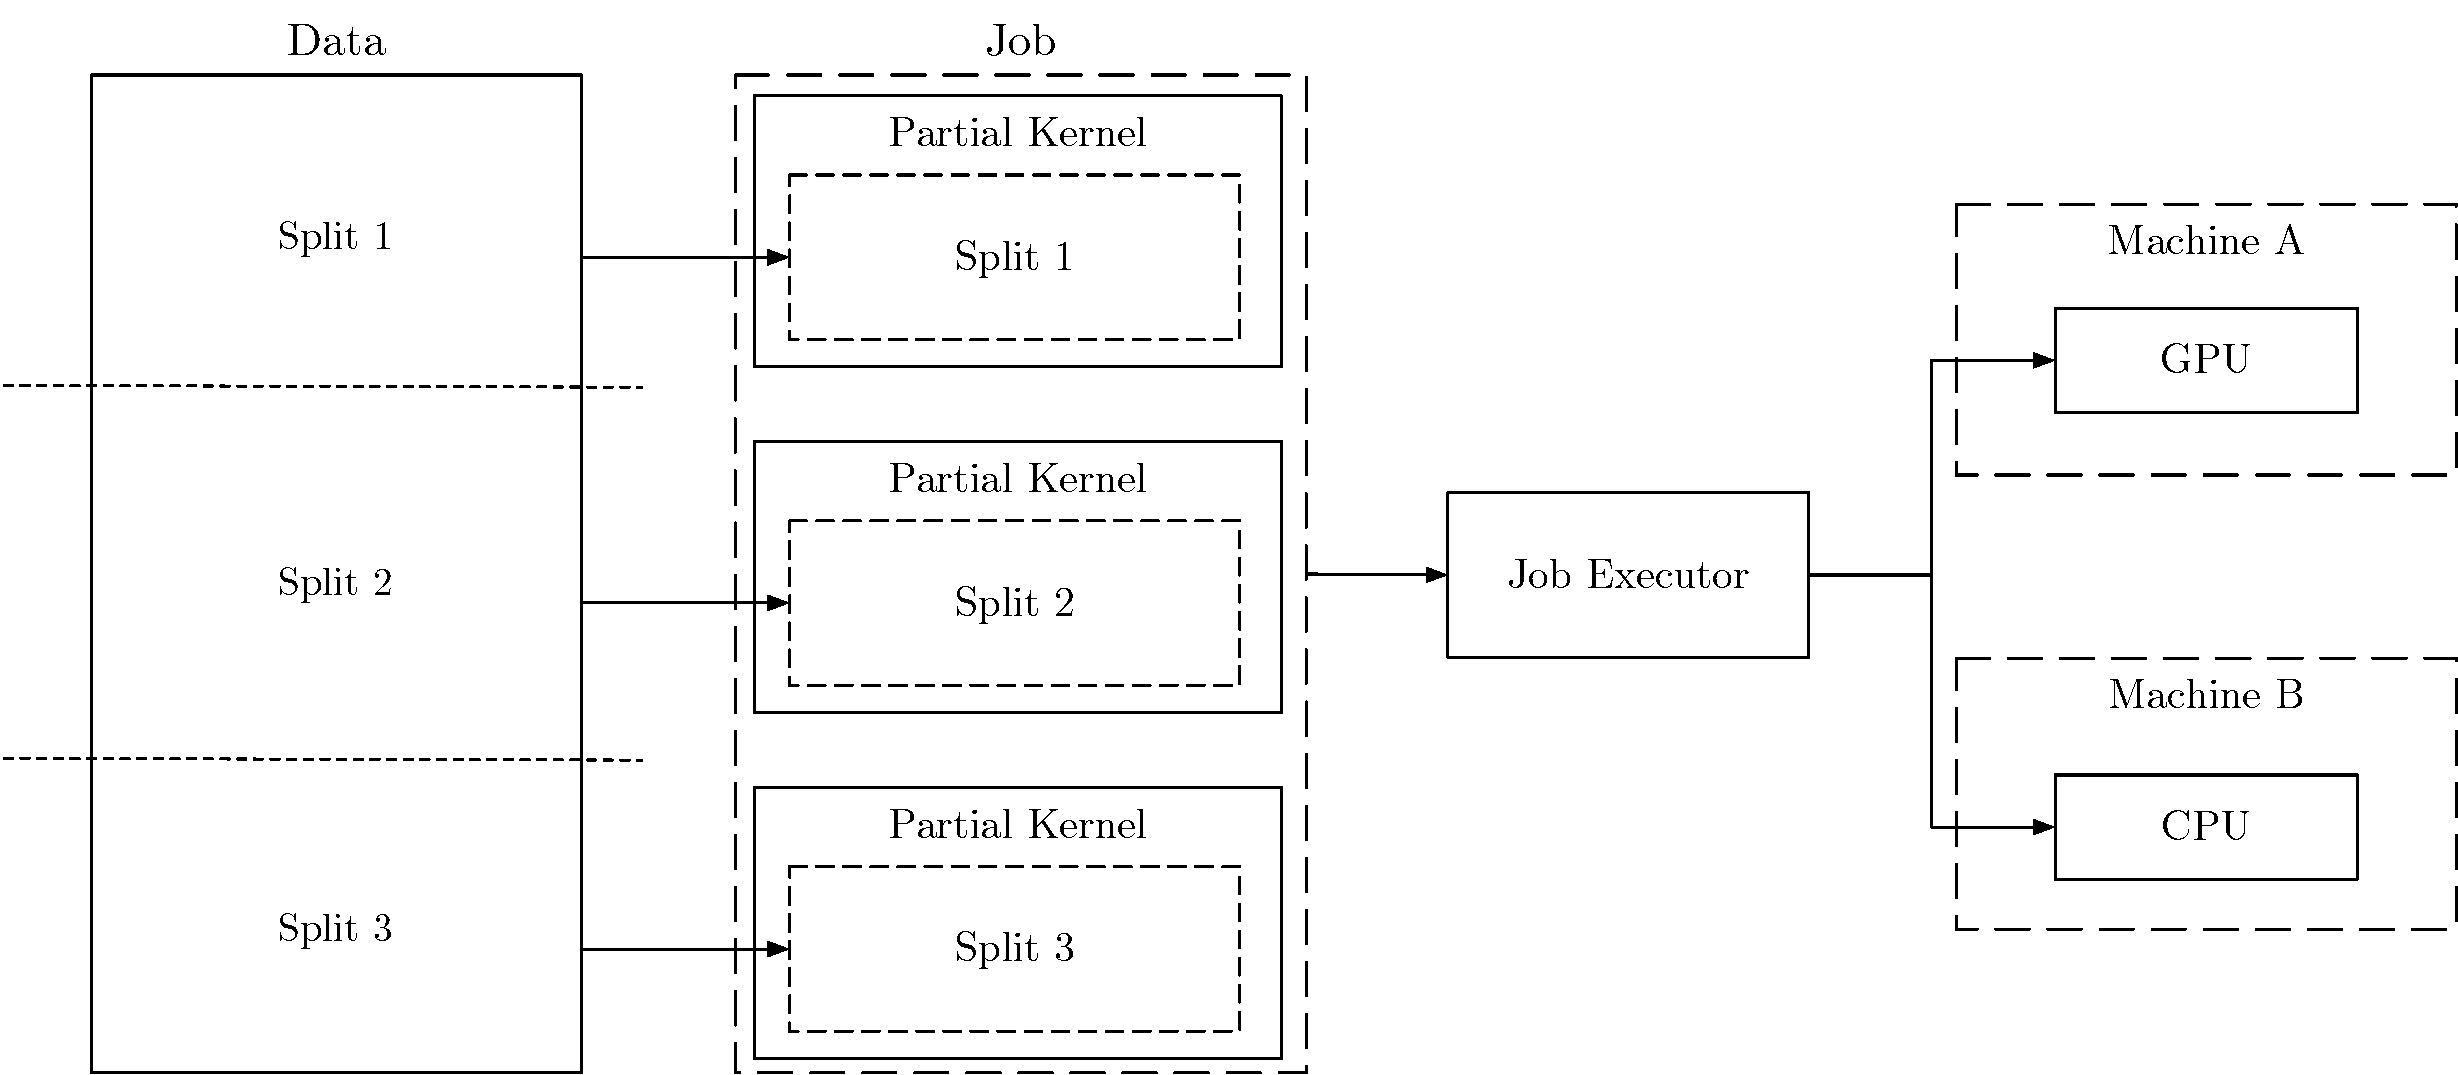
\includegraphics[width=0.95\textwidth]{drawings/dynamic_opencl_job.pdf}
	\centering
	\caption{Dynamic OpenCL Job Structure}
	\label{img:dynamic_opencl_job}
\end{figure}


\section{Hybrid Cloud}
\label{main_hybrid_cloud}
In the previous sections benchmarks and code examples were shown based on the existence of a local cluster. Such setups may provide cheap and stable performance when completely utilized. In reality resource demands fluctuate, making it hard to reach an equilibrium with a full resource utilization and no jobs being queued. For instance, the New York University published monthly utilization measurements for their three clusters in 2013\cite{nyu}, which are shown as a yearly aggregate in table \ref{table:cluster_utilization}. Aside from visible differences in average utilization all clusters show a considerably high standard deviation.

\begin{table}[!htb]
	\centering
	\begin{adjustbox}{width=0.5\textwidth}
		\small
		\begin{tabular}{l | l | l | l}
			~						& \textbf{Cluster 1}	& \textbf{Cluster 2}	& \textbf{Cluster 3}                 \\
			\hline
			\textbf{Average Utilization} 	& 81.1\%  	& 71.0\% 	& 76.1\% \\
			\textbf{Std. Deviation}          & 5.2\%  	& 4.9\%		& 16.9\% \\
		\end{tabular}
	\end{adjustbox}

	\caption{NYU Cluster Utilization}
	\label{table:cluster_utilization}
\end{table}

When providing a shared cluster that can be used by multiple parties, certain trade-offs apply. On the one hand overprovisioning decreases waiting times for users but increases costs. On the other hand underprovisioning reduces costs but comes with the price that users may have to line up in queues to access resources. In order to counter this imbalance, remote cloud machines could be employed, which can be booked and released dynamically and are billed hourly or even minutely. Among the most prominent services are Amazon's EC2, Microsoft's Azure and Google's App Engine. While each of these cloud services has its advantages and disadvantages, EC2 is the only that has bookable GPU instance types at various sizes. Although Azure and App Engine also have similar offerings, they are either only available as a preview in limited regions or can only be accessed by companies. Therefore, EC2 is used as the exemplary cloud service for this research but with interchangeability in mind so that it is possible to replace EC2 with other services in the future.

Interconnecting the framework with EC2 requires including the AWS software development kit (abbr. SDK), which is available for Java among many other languages. Through the SDK, the API for reserving and releasing instances can be accessed. Additionally, an Amazon Machine Image (abbr. AMI) is required so that newly launched instances will have OpenCL installed and run the dOpenCL daemon by default on startup. For this cause an Ubuntu 14.04 based image was created with the appropriate drivers and dOpenCL installed, which is started right after booting the machine.

Adding and releasing machines within the framework shall be handled by a class called \textit{Machine Manager}, abstracting the actual implementation of the utilized SDK in order to enable users to interchange the underlying cloud provider:


\begin{lstlisting}[caption=Machine Manager Abstract Implementation,captionpos=b]
public abstract class MachineManager {
  protected abstract List<DynamoInstance> bookInstance(int count, String type);
  protected abstract void terminateInstances(List<DynamoInstance> instances);
  ...

  public List<DynamoInstance> book(int count, String type){
    List<DynamoInstance> instances = bookInstance(count, type);
    ...
    return instances;
  }

  public void release(List<DynamoInstance> instances){
    terminateInstances(instances);
    ...
  }
}
\end{lstlisting}

The above code shows the abstract class that handles bookings and releases of instances in the context of dOpenCL. In the actual implementation it includes functionalities which ensures that the booked instances are successfully booted and running the dOpenCL daemon before adding them to the cluster as well as removing them. These pieces have been deducted for the sake of readability. The actual implementation of the \textit{EC2 Machine Manager} fills the abstract methods in which it accesses the Amazon SDK for booking and releasing machines. In order to employ another cloud provider, a class that implements the abstract methods for calling the respective cloud API has to be created.

An important factor to consider when connecting a local cluster with a remote cloud is security. Remote machines should be sufficiently secured to prevent attackers from taking over machines or utilizing resources via calling the running dOpenCL daemon. By default the EC2 Ubuntu images only allow certificate based SSH, which prevents password attacks on any account. Additionally, Amazon offers the management of Security Groups that put machines behind a virtual firewall. Therefore the security group can be configured to only allow packages from the static IP range of the local cluster, which renders attacks from outside of the local network useless. Any newly booked instance will be included within the Security Group and are therefore protected.

\section{Scalable Performance}
\label{scalable_performance}
In section \ref{job_design} the general job design was explained that is employed in Dynamic OpenCL. As jobs may contain an arbitrary number of partials, the number of partials determines the maximum potential for parallelization. For example a matrix multiplication that has been split into four partials may be computed by four devices in parallel. Following Amdahl's law it can benefit from a maximum 4x times speedup\cite{amdahl}, assuming minimal sequential portions of code. In reality the sequential portions are affected by central scheduling mechanisms and data transfers, reducing the potential of speedups significantly. Thus, choosing the appropriate number of partials is influenced by a performance trade-off: while an increased number of partials per job allows to utilize more devices in parallel and as such a potentially higher performance, each partial has to be scheduled by the framework and started in its own OpenCL Kernel. Starting the Kernels in parallel may lead to network congestions, diminishing remaining speedup potential. Therefore it might be beneficial for certain jobs to keep the number of partials lower than the number of available devices in the cluster in order prevent performance penalties through overheads and bottlenecks.

The general idea behind scaling performance within the framework is based on booking additional resources through a remote cloud when demand is high. Similarly, in the case of low demand resources can be released again in order to minimize costs. Widely employed cluster resource management solutions like Hadoop Yet Another Resource Negotiator (abbr. YARN) include functionalities to add or remove nodes dynamically. In a YARN cluster each node is independent and communicates with a central master node that keeps track of utilized resources and handles each compute node as an individual entity. Offering a similar functionality in a dOpenCL based solution differs substantially.

OpenCL and Aparapi are built to run on a single machine and as such include assumptions of limited capabilities concerning changing hardware during operation. For example Aparapi caches device queries to OpenCL as devices are usually added or removed during maintenance procedures when a machine is powered down. dOpenCL overcomes such limitations and enables the central machine to have devices virtually installed by adding nodes to the dOpenCL cluster. dOpenCL therefore extends the OpenCL standard by adding the custom methods \textit{clCreateComputeNodeWWU} and \textit{clReleaseComputeNodeWWU}.

As OpenCL itself has no multi-machine capabilties it only offers information for the respective built-in devices through the standard API. Therefore all devices appear as if they were installed in the central machine that runs the dOpenCL library. This makes identifying the owning machine per device impossible. Knowing the relation between devices and machines is crucial for providing basic functionality like releasing superfluous machines, where it has to be ensured that no partials are running anymore on a respective machine. In order to provide the machine-device relation dOpenCL introduces another method called \textit{clGetDeviceIDsFromComputeNodeWWU}.

The mentioned dOpenCL methods are available to C++ programmers when including the respective header files that contain the extensions. Thus, host code that wants to benefit from dynamic device management has to be modified appropriately. In its standard version Aparapi is bound to the standard OpenCL specification and has no understanding of the offered dOpenCL extensions. Therefore it is necessary to modify the Aparapi JNI to enable dynamic resource scaling. In order to do so, two new JNI methods are introduced, \textit{addNode} and \textit{removeNode}. Both call the respective dOpenCL functions, with \textit{addNode} also reporting back the available devices of the added node.

\section{Optimized Scheduling}
\label{optimized_scheduling}
As Dynamic OpenCL is supposed to offer its services to variously structured jobs in parallel, scheduling considerations have to be undertaken to maximize the overall system efficiency and ensure a fair resource sharing process. It must be understood that both requirements can be contradictory depending on the submitted workloads and heterogeneity of available devices. In certain cluster setups scheduling decisions based on fairness could result in partials being assigned to inadequate devices. For example a job that runs especially well on GPUs could receive a CPU device, thus lowering the overall efficiency. On the other hand, considering only performance based factors might starve certain jobs until all other workloads have finished.

In order to allow the scheduler to adapt to specific cluster requirements, a pluggable two tiered architecture is proposed. As such the scheduler consists of two modules, called \textit{Job Scheduler} and \textit{Device Scheduler}. Both modules are implemented following a defined Java interface, thus allowing interchangeability. This allows users to program their own scheduling algorithms and place them in the scheduler. Additionally Dynamic OpenCL allows switching out the modules during runtime in order to enable clusters to adapt to varying situations and usage scenarios. The overall scheduling architecture is depicted in figure \ref{img:scheduling_arch}. In the following sections the Job Scheduler and Device Scheduler are explained in detail.

\begin{figure}[!htb]
	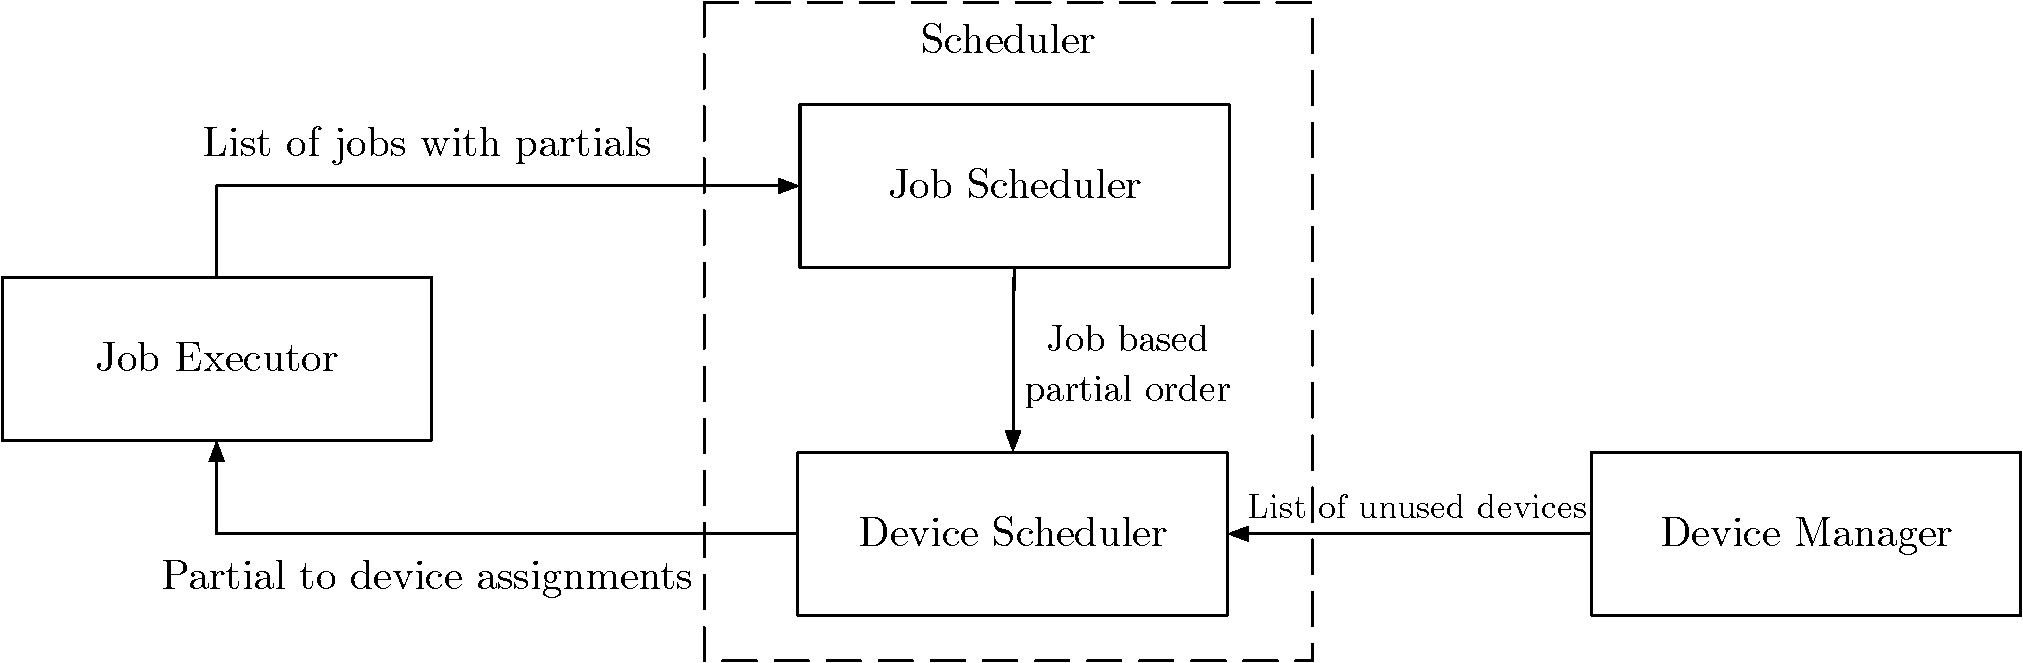
\includegraphics[width=0.95\textwidth]{drawings/scheduling_arch.pdf}
	\centering
	\caption{Scheduling Architecture}
	\label{img:scheduling_arch}
\end{figure}

\subsection{First Tier: Job Scheduler}
The first scheduling tier only considers the system state on a job abstraction level without having any knowledge about the actual partial structure or available devices in the cluster. Instead this tier is mainly concerned about ensuring predefined fairness policies and as such controls the order in which jobs are eligible for consideration during a scheduling round. Algorithms available in Dynamic OpenCL for this tier are the following:

\begin{description}[style=nextline]
	\item[First-In First-Out (abbr. FIFO)]
	Jobs are fully prioritized by their submission time. Thus, partials of two jobs will be completely submitted sequentially with the older job coming in front. Example: Job A with two partials a and Job B with four partials b will lead to the order aabbbb.
	\item[Round-Robin]
	Tasks are put equally in rotating order so that each job gets a fair share of resources. Example: Job A with two partials a and Job B with four partials b will lead to the order ababbbb.
\end{description}

All of the above approaches do not require insight into the actual performance figures but determine the resulting partial order by high level attributes like job submission time etc. Moreover, the selected algorithm on this tier can lead to significantly different outcomes for the overall system due to severe variations in fairness. Still, the first tier only hands over the partial order to the second tier, which may choose to ignore the given order based on the nature of the underlying algorithm.

It must be noted that strict scheduling concepts like FIFO are handled in a relaxed manner in order to allow a better cluster utilization. For example a strict FIFO scheduler would only pass on partials of a single job to the next scheduling tier. This behavior is not recommended as the second scheduling tier may not find available devices that are appropriate for the single job. Instead job schedulers should compile a list of partials for all available jobs in their proposed order. This way the second scheduling tier can always assign partials to devices if prioritized jobs do not fit currently available devices.

\subsection{Second Tier: Device Scheduler}
The second scheduling tier gets its input from the preceding tier and has no concerns of the high level job abstraction. Instead it focuses on the actual assignment of partials to devices. Executing OpenCL code in a heterogeneous environment can lead to drastically different performance numbers based on the algorithm implementation and the executing device. For example code that may perform exceptionally well on a GPU may run poorly on a CPU because of varying computational capabilities. Therefore programmers are empowered in Dynamic OpenCL to express preferences in terms of the device types that their algorithm should be computed on. The mechanism is implemented through a defined \textit{Device Preference} attribute that can be attached to every partial. Valid values for the attribute include: \textit{None}, \textit{CPU only}, \textit{CPU preferred}, \textit{GPU only} and \textit{GPU preferred}. With these five preference levels programmers can accordingly specify their favorite device type. Using the \textit{CPU only} or \textit{GPU only} values signals algorithms to only assign the specific type. On the other hand \textit{CPU preferred} and \textit{GPU preferred} indicate that it is appropriate to schedule a GPU or a CPU respectively if the preferred type is not available. While it is possible for schedulers on this tier to ignore the defined preference, all currently implemented solutions within Dynamic OpenCL adhere to the specification.

It must be noted that algorithms on the second tier may utilize strongly varying approaches to assign partials to devices. While it might be feasible in certain environments to randomly send partials to devices, more thoughtful approaches may improve the overall efficiency of the system. As more analytical algorithms are likely to focus on performance indicators, the most promising options are explained and evaluated based on their eligibility.

For decades it has been a significant challenge to foresee execution times of algorithms on a given system. Execution times are especially crucial in real time systems such as cars, airplanes or space probes where it is mandatory to ensure that an algorithm finishes under a specified boundary, called worst case execution time (abbr. WCET). In order to obtain such timings one may employ various methods such as static code analysis or simulations\cite{wcet}.

In static code analysis algorithms are taken apart for the purpose of predicting control flow features such as loop counts without executing the actual code\cite{loopbound}\cite{sweet}. While there are formal approaches to gain insights about the executable instructions, estimating the running time is another great challenge. As modern processors have become increasingly complex due to the introduction of caches, pipelines and multi core architectures, instruction times may vary significantly\cite{wcet}. In the light of OpenCL this step becomes even more difficult through the availability of different device types and vendors, which inherit distinct architectures.

Simulations allow to draw conclusions about algorithm timings by running it on an abstract representation of the actual hardware\cite{wcet}. While \citeauthor{multi2sim} have proposed a framework for simulating CPUs and GPUs\cite{multi2sim}, the main drawback of such an approach is again the abundance of different hardware designs and architectures supported by OpenCL. In order to cover the majority of possible devices, many different simulators are required. For instance, each NVIDIA GPU architecture would demand a dedicated simulator.

While code analysis and simulation do not employ the actual hardware, benchmarks may be used to obtain indicators about the performance of a specific device for a given partial. For instance, \citeauthor{quantitative_performance} have proposed a model in which they measure key performance indicators like buffer bandwidth of a GPU\cite{quantitative_performance}. These measurements are then used to predict execution times of Kernels based on the identified bottlenecks by analyzing the instructions at hand. Other approaches run the Kernels with varying parameters in order to infer the dominant performance factors\cite{gpgpu_performance}. In all cases the methods are not universally transferable to other hardware architectures but have to be adjusted manually or utilizing machine learning.

All of the presented approaches are promising in their respective field of application. Still, the major limiting factor is the apparent focus on a specific hardware architecture, which makes the approaches unsuitable in the context of OpenCL. In order to cover all supported devices many different models would have to be employed, with each upcoming hardware architecture also introducing new models to Dynamic OpenCL. 

With the distribution of partials across a network not only the performance of the execution devices matters but also the speed of the network connection itself. This becomes especially important when utilizing resources from a distant cloud, which inherently can not offer the same bandwidth and latency as a local network. For example, in a benchmark a local cluster with 10 Gbit/s interconnects installed can only reach bandwidths of 190 Mbit/s when communicating to a low priced EC2 instance. Still the EC2 instance is able to transfer data at the speed of ~800 Mbit/s within the local EC2 cluster. Thus both machines perform well in their respective local network but the interconnection through the internet becomes the bottleneck. Such asymmetric connections could significantly affect data intense Kernels where the data transfers might exceed computation times on a slow connection. Thus, sending such Kernels to a high performance cloud device could be slower than sending it to a low performance local machine.

A naive approach that combines both measurements for device performance as well as network performance is the usage of historical data. With the assumption that jobs are split in many equally sized partials one can presume the best suited device of a Kernel from previous executions on various devices within the cluster. As Dynamic OpenCL schedules only a single partial on a device at a time, partials do not interfere with one another performance wise. Therefore the execution time of a Kernel is not affected by other Kernels and should accordingly remain stable across multiple runs. This behavior could also be observed during the benchmarks in section \ref{distribution} and \ref{abstraction} where multiple runs of the same Kernel showed little standard deviations.

In order to offer algorithms on the second tier valuable data, several analytical features are added to Aparapi and Dynamic OpenCL:
\begin{description}[style=nextline]
	\item[Kernel Data Size]
	Aparapi is extended by adding a method to the Kernel class that reports back the actual size of the overall Kernel including its data. The size is gained by employing Java reflection on a Aparapi Kernel, identifying used data types and data structures. As Aparapi offers explicit memory management not all of the data of a Kernel must be transferred. Therefore the returned size can only act as an approximation for the real amount of transferred data.
	\item[Historical Data Transfer]
	While knowing the exact amount of transferable data beforehand in the context of explicit memory management requires extensive code analysis, retaining these values in the aftermath of a Kernel execution is feasible. For this cause the memory management calls of Aparapi are modified to accumulate the sizes of the corresponding data structures in a Kernel attribute. With this functionality the total amount of transferred data is available after a Kernel has been executed. Then the attribute can be utilized by schedulers to conclude decisions for future Kernels of the same job.
	\item[Performance Cache]
	Dynamic OpenCL implements a mechanism to retain execution times of Kernels for every device they are run on. The observed timespan reaches from the deployment of the Kernel from its host code until the end of execution, thus including network transfers. Therefore the measurement takes into account different locations of the devices within the network. This means that a cloud device should yield slower execution times than an identical local device due to the data transfer penalties. With the resulting data, schedulers can come to decisions based on individual devices or even draw conclusions for devices of the same model.
\end{description}

In the current version of Dynamic OpenCL the most basic device scheduler available is the \textit{Device Preference Scheduler}, which only considers the respective device preference flag attached to a partial without any further performance considerations.
Based on the implemented \textit{Performance Cache} the \textit{Performance Based Device Scheduler} is also included. It assigns the currently available device with the best historical performance to a partial. With the available features concerning data transfer analysis more sophisticated and fine grained schedulers are possible to be implemented in the future. Additionally, system wide optimizations are feasible, which minimize the overall execution time of all submitted partials. For instance, a \textit{simplex} algorithm based scheduler would take into account trade off scenarios where it is beneficial not to grant a partial its best suited device but minimize the expected execution time among all scheduling decisions.

It must be noted that schedulers on this tier may rightfully ignore the order of partials given by the first tier. For example the first tier might hand over a list of partials in FIFO order. If this list is handled by a simplex based scheduler on the second tier, the principle of FIFO may be violated in favor of finding the optimal distribution.

\section{Exemplary Use Cases}
\label{use_cases}
In the previous sections the main characteristics of Dynamic OpenCL were explained. The included features make it a viable option for a variety of use cases which will be introduced in the following.

\begin{description}[style=nextline]
	\item[Job Based Library]
	One use case for the framework is to utilize it as a Java library for a single job thus keeping management overhead minimal. Programmers can either transform OpenCL code from C or C++ to Dynamic OpenCL or adapt already existing Aparapi code. In theory an Aparapi Kernel can be attached to a Dynamic OpenCL job without any changes. In fact such a job would not sufficiently utilize the provided partial mechanism. In order to enable parallelization, programmers are mandated to split their jobs into multiple partials to grant speedup potential.

	With the focus on a single job Dynamic OpenCL can schedule the submitted partials across a given cluster and report back results. As there are no other jobs to interfere, no extensive scheduling is required and all resources can be freely assigned to the job at hand. In the case of an execution that is slower than expected, users may book additional resources from an implemented cloud service and therefore reduce overall execution time in return for higher costs.

	\item[Local Cluster Provider]

	Instead of only acting on behalf of a single job, programmers can utilize Dynamic OpenCL to offer a shared platform for users to submit their jobs to. This becomes especially meaningful in the light of daily recurring jobs that only have to be programmed once. The platform could allow users to submit data to predefined jobs that take care of splitting the data into meaningful partials. Therefore users can profit from parallelization on powerful hardware without having programming knowledge on their own.

	The main limitation of the local cluster provider is its restriction to local resources only. Therefore the platform can not dynamically book instances from a cloud provider and with that increase the overall capabilities of the cluster. Running a shared platform on a local cluster may require some performance based scheduling in order to optimize resource assignments based on the running jobs.

	\item[Hybrid Cloud Provider]
	Local clusters may lead to phases of overprovisioning when resource demands by users are low, thus causing costs without any return in computation. In order to provide a more dynamic infrastructure Dynamic OpenCL can be used to guarantee a baseline of performance through local resources and add devices to the cluster from a cloud service when needed. While cloud devices may be more costly than local resources they can assist during peak demands and be released afterwards. Hence the overall costs of using a cloud resource may be lower than operating an underutilized local device.

	Additionally, volatile hardware requirements may lead to high total costs of ownerships. For instance, if only one job per month requires a GPU for efficient execution, installing a GPU in the local cluster might be costly. Instead such resources could be employed on demand whenever a job with such requirements is submitted.

	The main drawback of a hybrid cluster is the interconnection between both clusters that may suffer from low bandwidths. Therefore scheduling algorithms should be utilized that take the hybrid infrastructure into account and assign partials accordingly.

	\item[Cloud Cluster Provider]
	While hybrid clusters unite a static performance baseline with dynamic adjustments based on demand, a completely dynamic infrastructure is also possible. Instead of having computational resources running at all times, cloud clusters may only run a single management node. This central node receives jobs and orders new cloud resources depending on the actual demand. At times of no demand the management node runs alone, hence producing minimal costs.


\end{description}
